%%%%%%%%%%%%%%%%%%%%%%%%%%%%%%%%%%%%%%%%%%%%%%%%%%%%%%%%%%%%%%%%%%%%%%%%%%%%%%%%
%2345678901234567890123456789012345678901234567890123456789012345678901234567890
%        1         2         3         4         5         6         7         8

\documentclass[letterpaper, 10 pt, conference]{ieeeconf}  % Comment this line out if you need a4paper

%\documentclass[a4paper, 10pt, conference]{ieeeconf}      % Use this line for a4 paper

\IEEEoverridecommandlockouts                              % This command is only needed if 
                                                          % you want to use the \thanks command

\overrideIEEEmargins                                      % Needed to meet printer requirements.



% See the \addtolength command later in the file to balance the column lengths
% on the last page of the document

% The following packages can be found on http:\\www.ctan.org
%\usepackage{graphics} % for pdf, bitmapped graphics files
%\usepackage{epsfig} % for postscript graphics files
%\usepackage{mathptmx} % assumes new font selection scheme installed
%\usepackage{times} % assumes new font selection scheme installed
\usepackage{amsmath} % assumes amsmath package installed
\usepackage{amssymb}  % assumes amsmath package installed
\usepackage{accents}
\usepackage{graphicx}
\usepackage[font=small,labelfont=bf]{caption}
\usepackage{subcaption}
\usepackage{float}
%\usepackage{framed}
\usepackage{cite}
\usepackage{algorithm}
\usepackage{algorithmic}

% Some table tweaks to increase spacing
%\setlength{\tabcolsep}{8pt}		% Default is 6pt
\renewcommand{\arraystretch}{1.2}	% Default is 1.0


%%%%%%%%%%%%%%%%%%%%%%%%%%%%%%%%%%%%%%%%%%%%%%%%%%%%%%%%%
\title{\LARGE \bf
	Explosive Motion with Compliant Actuation Arrangements in Articulated Robots
}



%%%%%%%%%%%%%%%%%%%%%%%%%%%%%%%%%%%%%%%%%%%%%%%%%%%%%%%%%
\author{Roel Djajadiningrat$^{1}$, Wesley Roozing$^{2}$ and Nikolaos G. Tsagarakis$^{2}$% <-this % stops a space
	\thanks{$^{1}$ Roel Djajadiningrat is a M.Sc student at the Department of Mechanical Engineering, TU Delft and a visiting student at Istituto Italiano di Tecnologia;
		{\tt\ r.djajadiningrat@student.tudelft.nl}
	}%
	\thanks{$^{2}$Wesley Roozing and Nikolaos G. Tsagarakis are with the Department of Advanced Robotics,
		(Fondazione) Istituto Italiano di Tecnologia, via Morego,
		30, 16163 Genova, Italy.
		{\tt\ \{wesley.roozing, nikos.tsagarakis\}@iit.it}
	}%
}


%%%%%%%%%%%%%%%%%%%%%%%%%%%%%%%%%%%%%%%%%%%%%%%%%%%%%%%%%
\begin{document}

\maketitle
\thispagestyle{empty}
\pagestyle{empty}


%%%%%%%%%%%%%%%%%%%%%%%%%%%%%%%%%%%%%%%%%%%%%%%%%%%%%%%%%
\begin{abstract}

This paper presents the optimisation of joint trajectories and elastic element pretension for jumping of a 3-DoF leg prototype. The leg is based on the recently introduced asymmetric compliant actuator scheme, in which a series-elastic main drive is augmented in parallel with a secondary adjustable compliant branch with significantly different stiffness and energy storage capacity properties. The leg prototype implements two such actuation configurations, one of which includes a biarticulated branch, and they are compared to a conventional series-elastic based actuation structure. An optimisation problem is formulated to optimise the joint trajectories and elastic element pretension to maximise jumping height. The results demonstrate that the biarticulated configuration yields maximum jumping height, and achieves the highest peak joint power. Compared to series-elastic based actuation, the augmented leg jumps 4\% higher with a monoarticulated parallel compliance configuration while using less energy, and over 10\% higher in biarticulated configuration.

\end{abstract}


%%%%%%%%%%%%%%%%%%%%%%%%%%%%%%%%%%%%%%%%%%%%%%%%%%%%%%%%%
\section{INTRODUCTION}
In the past robot applications were found predominantly in static industrial settings, but over the past years robots have been introduced to more dynamic settings, operating with and among humans. This change in application is accompanied by a change in requirements of robots. One of the primary challenges today is letting robots match human-like behaviour in terms of motion. This requires light-weight actuation systems that allow for energy efficient explosive motion, large instantaneous forces with short duration, and matching motion planning and control. A prime example of an explosive motion in humans is the vertical jump.

Several approaches have been investigated over the years to design robotic systems capable of energy efficient explosive motion. Traditional rigid actuation poses problems with weight and resulting insufficient performance. Therefore, systems with compliant properties have been proposed. The compliant `Bow Leg' hopping robot \cite{zeglin1999bow} used a curved leaf spring made of laminated fibreglass, and showed that low power motors can be sufficient active actuation when parallel energy storage is used. A small bipedal jumping robot `Mowgli' \cite{niiyama2007mowgli} used compliant tendons antagonistic to pneumatic artificial muscles, enabling it to jump as high as 0.5\,m. A switchable form of Parallel-Elastic Actuation (\textit{PEA}) was shown to combine the benefits of compliant properties while maintaining a high degree of control and energy efficiency when the parallel compliance is not needed \cite{liu2015spear}. Besides actuation parameters, the importance of optimised joint trajectories was shown to be a major factor in improved energy efficiency \cite{velasco2013soft, babivc2009biarticulated}. Furthermore, biarticulated actuation, in which a single muscle spans multiple joints simultaneously, has been shown to drastically increase explosive performance in humans \cite{schenau1989rotation,prilutsky1994tendon}. In robotics, comparative jumping experiments with single-actuator biarticulated robots and multiple-actuator robots also demonstrate increased performance of biarticulated configurations \cite{oshima2007jumping,babivc2009biarticulated,hyon2002development}.

% some old sentences we don't have space for
% It was shown that accurate and stable force control can be achieved with Series Elastic Actuation (\textit{SEA}) \cite{pratt1995series}.
% Analytical research on Series-Elastic Actuation (SEA) shows that a \textit{SEA} performing a hammering task can reach a speed up to four times that of the actuator’s prime mover \cite{garabini2011optimality}.
%A comparison with \textit{PEA} showed that a hopper with \textit{SEA} is more energetically efficient than one with \textit{PEA} when looking at positive actuator work and electrical work \cite{yesilevskiy2015comparison}.

Recently, Roozing et al. \cite{roozing2016development, roozing2016design, roozing_design_2018} presented the development and control of a novel Asymmetric Compliant Actuation (\textit{ACA}) scheme characterised by large energy storage capacity that enables efficient execution of motions, as well as a novel method to select the design parameters of such structures to maximise energy efficiency of multi-DoF articulated robots powered by this type of actuators. This paper extends these previous works, contributing by using the \textit{ACA} concept to execute optimised jumping motions on the model of the recently developed 3-DoF leg prototype \cite{roozing_design_2018}. Two augmented actuation designs, one of which includes a biarticulated tendon spanning ankle and knee, are compared to a state-of-the-art SEA-based actuation structure, demonstrating significant benefits of such actuation approaches in explosive motions.

This paper is structured as follows. Sec. \ref{sec:legDesign} describes the 3-DoF leg prototype, the actuation concepts, and the three different actuation configurations. Sec. \ref{sec:modelling} describes the forward and inverse dynamics of the leg. Sec. \ref{sec:dynamicOptimisation} introduces the optimisation problem, followed by the results in Sec. \ref{sec:results}. The paper concludes with a discussion of the results in Sec. \ref{sec:discussion} and conclusions in Sec. \ref{sec:conclusions}.


%%%%%%%%%%%%%%%%%%%%%%%%%%%%%%%%%%%%%%%%%%%%%%%%%%%%%%%%%
\section{Leg Design}
\label{sec:legDesign}

\subsection{Asymmetric Compliant Actuation}
\label{subsec:ACA}
The Asymmetric Compliant Actuation (\textit{ACA}) concept consists of a combination of two parallel actuation branches with very different power and stiffness properties, as shown in Fig. \ref{fig:ACA}. The Power Branch (\textit{PB}) is a rotary \textit{SEA} which consists of a high power motor \textit{M1} in series with a torsional elastic element \textit{SE}. The Energy Storage Branch (\textit{ESB}) consists of a lower power motor \textit{M2}, with a high reduction linear transmission which transfers its power to the joint through a unidirectional series elastic element \textit{PE}. In biarticulated configurations (bottom of Fig. \ref{fig:ACA}), the \textit{PB} drives the joint directly, while the \textit{ESB} tendon spans a second joint by means of a free pulley, as depicted in Fig. \ref{fig:ACA}. As such, the tendon elongation depends on the configuration of both joints, and the tendon exerts torque on both joints.

% Figure asymmetric compliant actuation branches
\begin{figure}[ht]
	\centering
	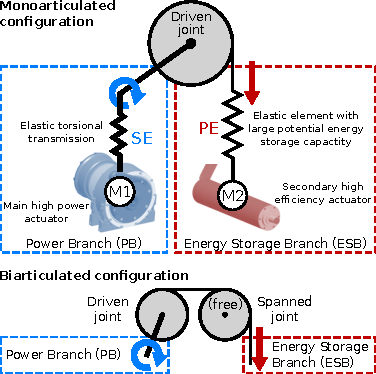
\includegraphics[width=0.8\linewidth]{actuationConcept}
	\caption{The Asymmetric Compliant Actuation (\textit{ACA}) concept, shown in monoarticulated (top) and biarticulated (bottom) configurations.}
	\label{fig:ACA}
\end{figure}

\subsection{3-DoF Leg Prototype}
The design of the 3-DoF leg prototype is inspired by the human lower limb. The dimensions and mass distribution of the human limb were investigated, and compared with those of existing humanoid designs such as WALK-MAN \cite{tsagarakis2017walk} to set specifications for a semi-anthropomorphic design. The leg features three actuated degrees of freedom: ankle, knee and hip. Each joint is directly actuated by an \textit{SEA}, which are mounted above the joints for the knee and ankle, and transmit their forces through four bar linkages to decrease the leg’s moment of inertia with respect to the hip joint. The trunk is loaded with mass corresponding to that of a full humanoid robot in two-legged stance. The leg can be rapidly reconfigured into one of three actuation configurations:

\begin{enumerate}
	\item \textbf{SEA-only} based actuation, in which the parallel Elastic Storage Branch is not implemented, serving as a baseline state-of-the-art design for comparison.
	\item \textbf{Monoarticulated} configuration, in which the knee and ankle joints are each augmented with an \textit{ESB}.
	\item \textbf{Biarticulated} configuration, in which the tendon for the ankle joint also spans the knee joint.
\end{enumerate}

Fig. \ref{fig:configurations} shows a schematic of the leg design in all three actuation configurations. Following the method presented in \cite{roozing2016design}, the design parameters each configuration were optimised to select actuation parameters that yield high electrical energy efficiency and reduction in peak torque and electrical power requirements. For more details on the hardware implementation, we refer the reader to \cite{roozing_design_2018}.

% Figure Actuation configurations
\begin{figure}[ht]
	\centering
	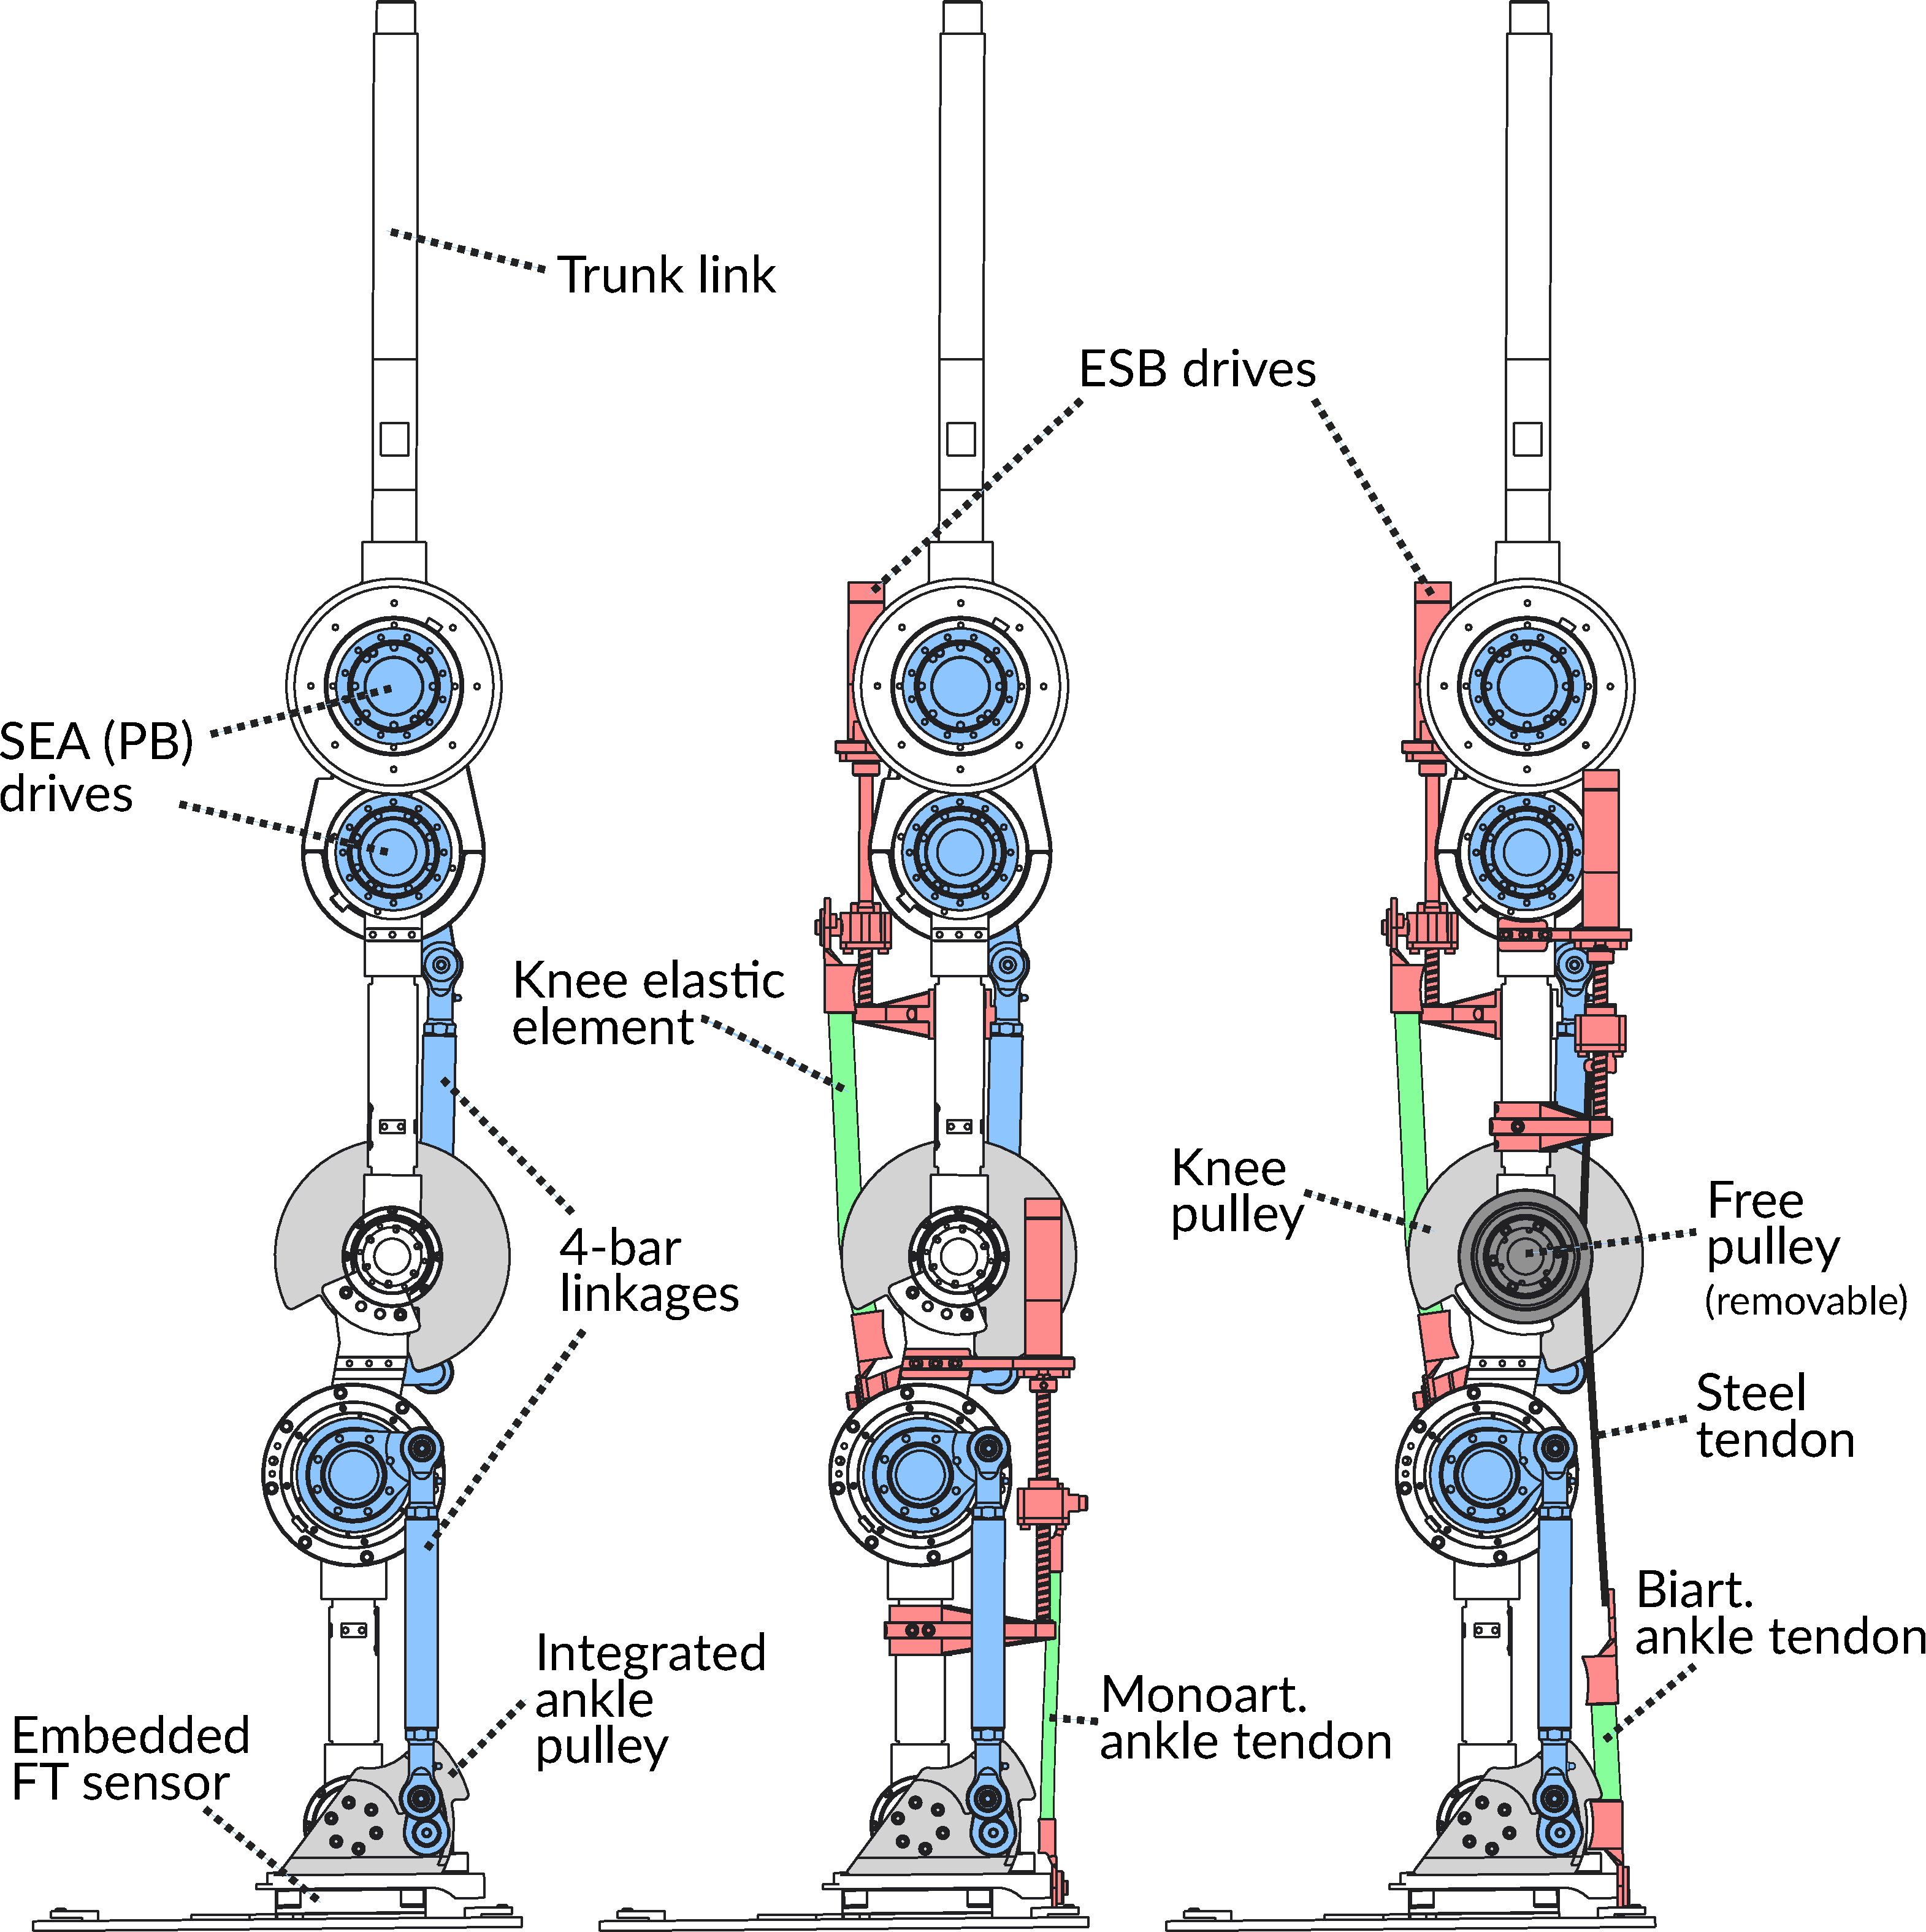
\includegraphics[width=0.98\linewidth]{cad}
	\caption{CAD: SEA-only, mono- and biarticulated configurations}
	\label{fig:configurations}
\end{figure}


%%%%%%%%%%%%%%%%%%%%%%%%%%%%%%%%%%%%%%%%%%%%%%%%%%%%%%%%%
\section{Modelling} 
\label{sec:modelling}

\subsection{Leg Model: Forward Dynamics} 
The leg consists of four links which are connected by the actuated ankle, knee and hip joints, denoted $q_1,q_2,q_3$, with net actuation torques $\tau_1,\tau_2,\tau_3$ as shown in Fig. \ref{fig:Leg_3DoF_model}. The links have masses $m_1,m_2,m_3,m_4$ and rotational inertiae $J_1,J_2,J_3,J_4$. Their centre of mass (CoM) is assumed to be located on the line connecting the proximal and distal joints at a distance of $r_1,r_2,r_3,r_4$ from the proximal joint for all links except for the foot; the model includes a floating base to allow for realistic modelling of the ground reaction forces (GRF). %Together, the configurations of the bodies describe the system:
%\begin{equation}
%	\mathbf{x} = [x_1,y_1,\theta_1,x_2,y_2,\theta_2, x_3,y_3,\theta_3,x_4,y_4,%\theta_4]^T. 
%\end{equation}
The Euler-Lagrange formulism with generalised coordinates $\mathbf{q} \in \mathfrak{Q} \subset \mathfrak{R}^{6}$ is used to derive the dynamic equations:
\begin{equation}
	\mathbf{q} = [x_1,y_1,\theta_1,q_1,q_2,q_3]^T,
	\label{eq:q}
\end{equation}
leading to:
\begin{equation}
	M(\mathbf{q}) \, \mathbf{\ddot q} = \mathbf{\boldsymbol{\tau}} + \mathbf{g}(q) - C(\mathbf{q, \dot q}) \, \mathbf{\dot q} - D \, \mathbf{\dot q} + J_{GRF}^T \, \mathbf{f}_{GRF}.
\label{eq:fwddyn}
\end{equation}

% Figure Leg model
\begin{figure}[ht]
	\centering
	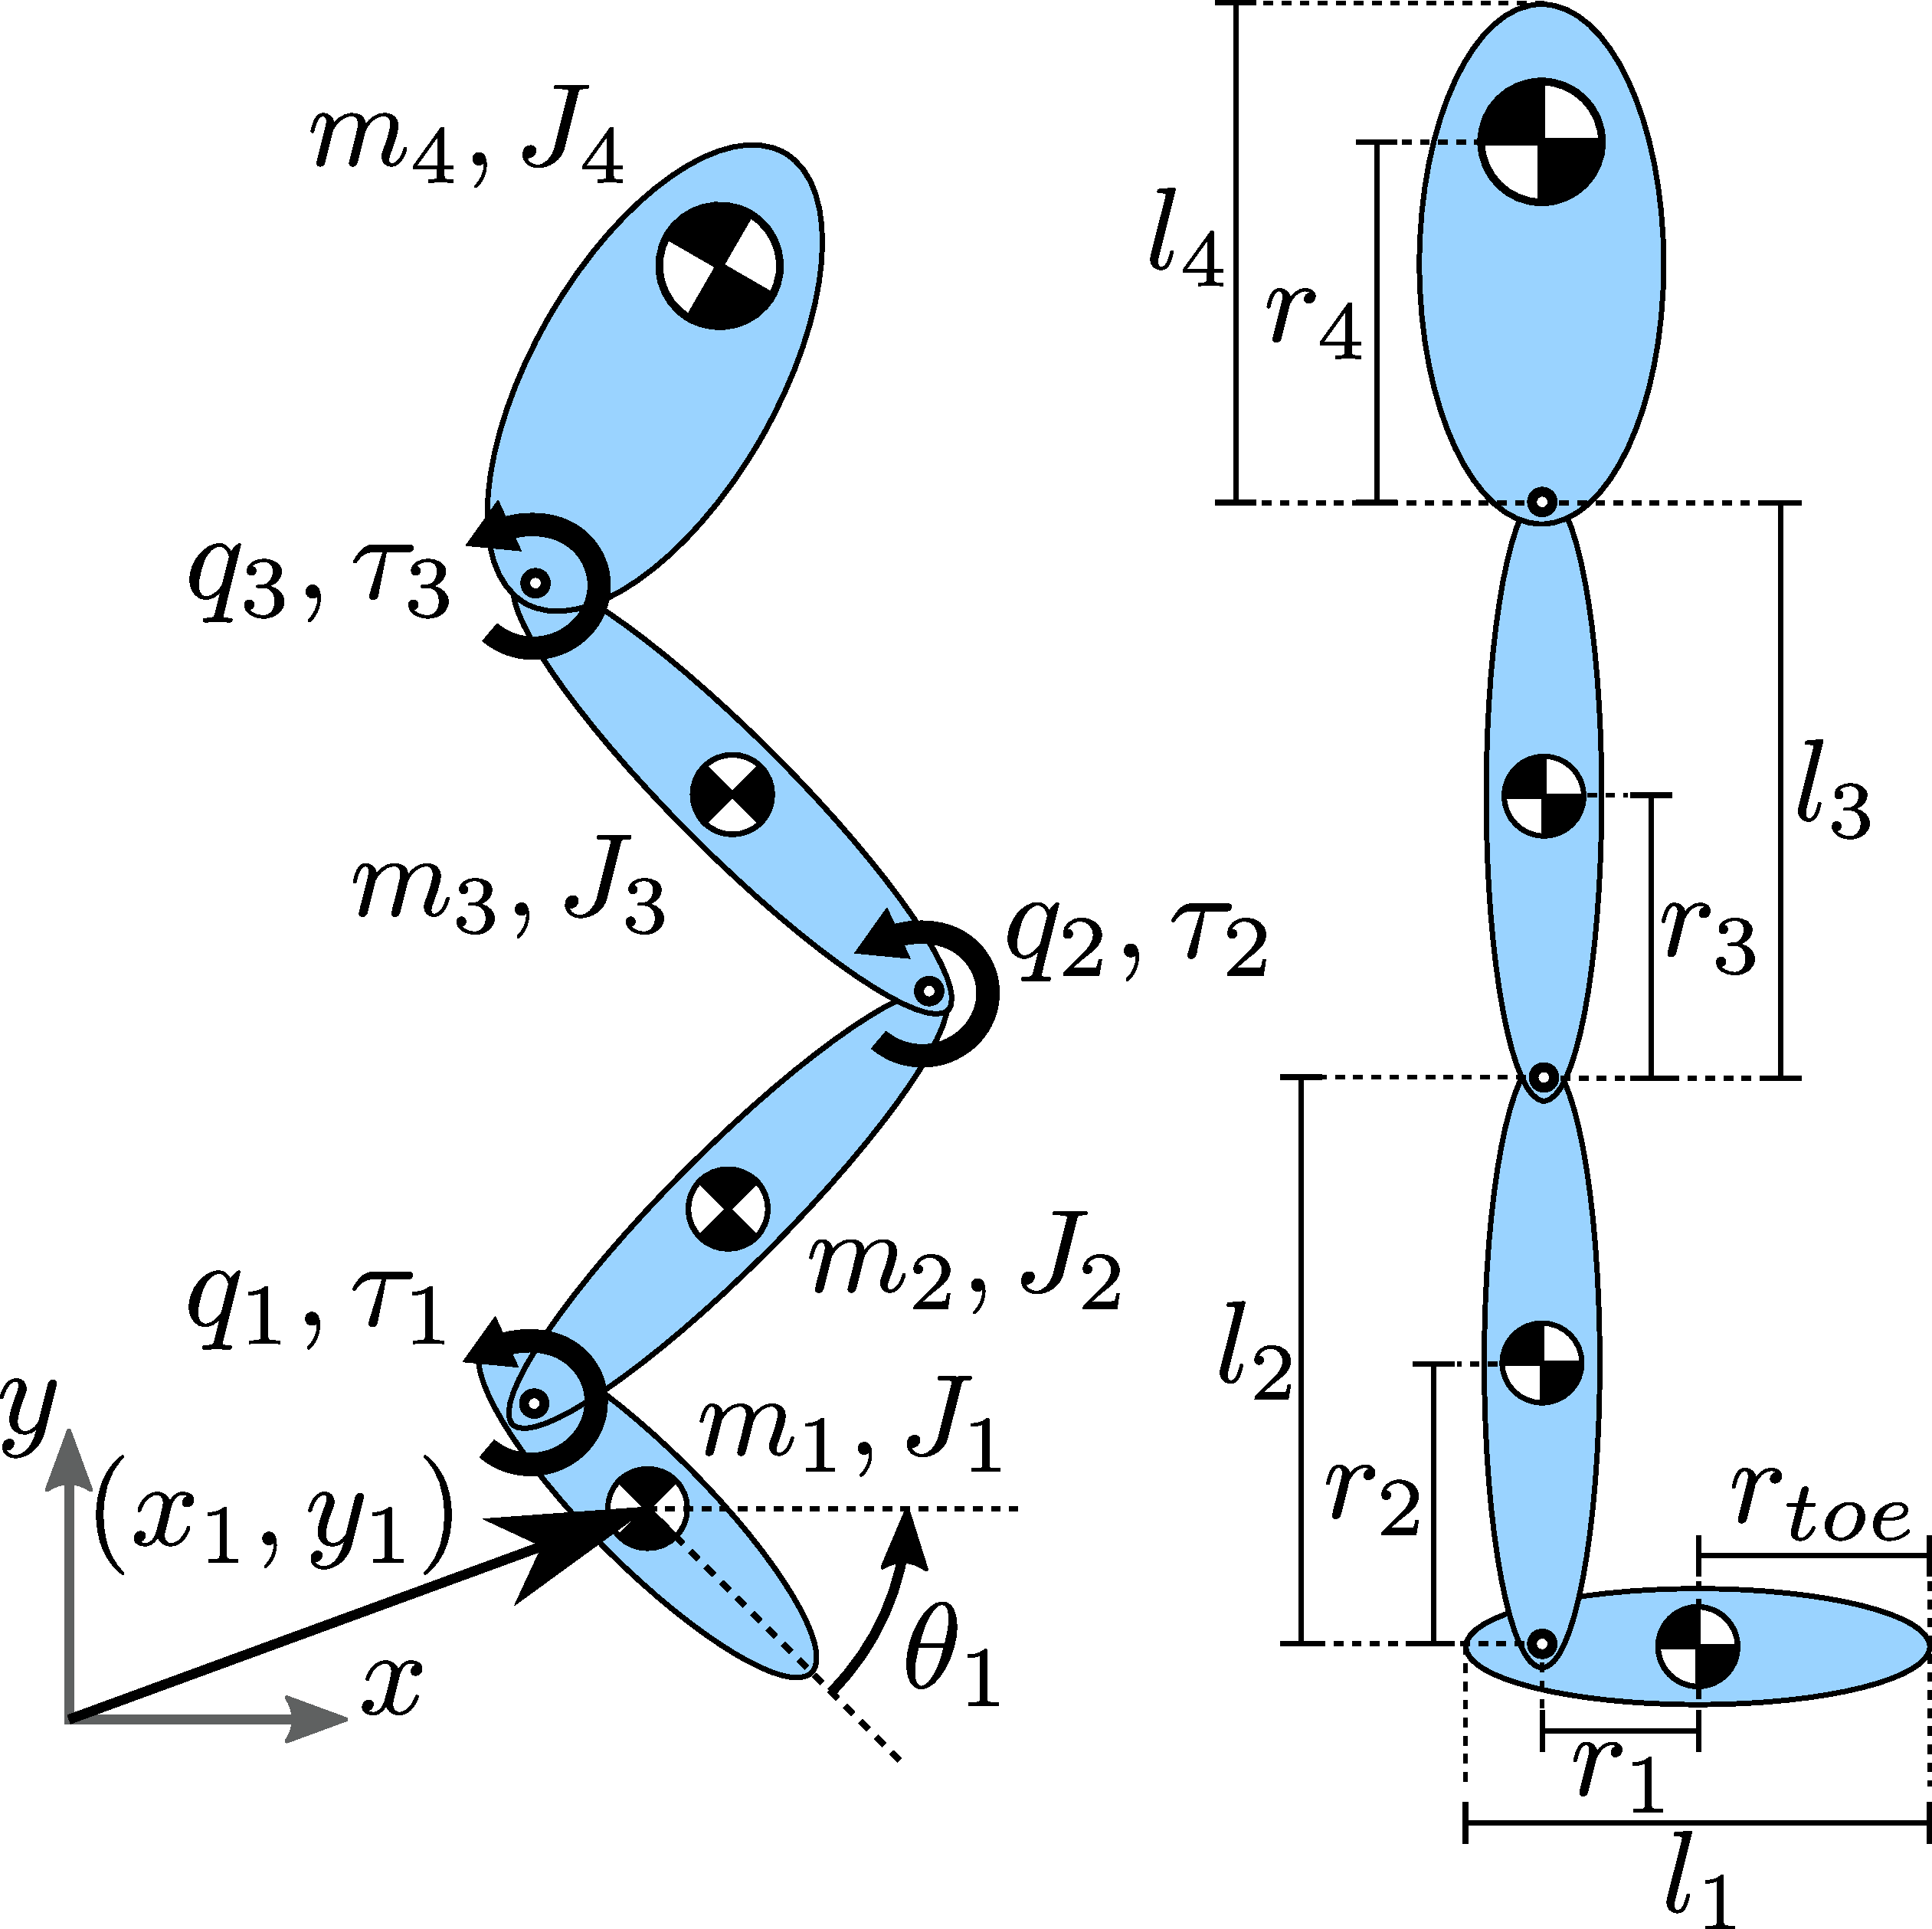
\includegraphics[width=0.6\linewidth]{Leg_3DoF_model}
	\caption{Leg model with floating base. The straight configuration on
		the right corresponds to $\mathbf{q} = \mathbf{0}$.}
	\label{fig:Leg_3DoF_model}
\end{figure}

Here, the damping matrix is denoted by $D = \mathrm{diag} (0,0,0,d_1,d_2,d_3)$, the generalised actuation forces are denoted by $\boldsymbol{\tau} = [0,0,0,\tau_1,\tau_2,\tau_3]^T$, the generalised gravitational forces are denoted by $\mathbf{g(q)}$, and the Coriolis and generalised inertia matrices are denoted by $C\mathbf{(q, \dot q)}$ and $M(\mathbf{q})$, respectively. The Jacobian for the heel and toe is denoted by $J_{GRF}^T$ and the ground forces in generalised coordinates are subsequently expressed as $J_{GRF}^T \, \mathbf{f}_{GRF}$. Spring-dampers define $\mathbf{f}_{GRF}$ in the vertical direction and Coulomb and viscous friction define the horizontal component, proportionally to the vertical forces.

\subsection{Leg Model: Inverse Dynamics}
For formulation of the optimisation problem described in Sec. \ref{sec:dynamicOptimisation}, we first derive the inverse dynamics of the system in order to compute the applied active torques \cite{nakanishi2007inverse}. The configuration vector $\mathbf{q}$ can be split in its passive and active joint components, $\mathbf{q}_p$ and $\mathbf{q}_a$, respectively:
\begin{equation}
\mathbf{q} =
\begin{bmatrix}
	\mathbf{q}_p \\
	\mathbf{q}_a
\end{bmatrix},
\end{equation}
with
\begin{equation}
	\mathbf{q}_p = [x_1,y_1,\theta_1]^T, \quad  
	\mathbf{q}_a = [q_1,q_2,q_3]^T.
\end{equation}
\noindent
Similarly, $\boldsymbol{\tau} = \left[\mathbf{0},\boldsymbol{\tau}_a\right]^T$. Substituting these into \eqref{eq:fwddyn} yields:
\begin{equation}
	\begin{aligned}
		&\left[\begin{array}{cc}  
		M_{pp} & M_{aa}\\
		M_{ap} & M_{aa}
		\end{array} \right]
		\left[\begin{array}{c}  
		\mathbf{\ddot q}_p\\
		\mathbf{\ddot q}_a
		\end{array} \right] +
		\left[\begin{array}{c}  
		\mathbf{b}_p \mathbf{(q,\dot q)}\\
		\mathbf{b}_a \mathbf{(q,\dot q)}
		\end{array} \right] 
		=\\
		&\left[\begin{array}{c}  
		\mathbf{0}\\
		\boldsymbol{\tau}_a
		\end{array} \right] 
		+
		J_{GRF}^T \mathbf{f}_{GRF} \, \mathbf{(q, \dot q)},
	\end{aligned}
	\label{eq:ik}
\end{equation}		
where $\mathbf{b}_p$ and $\mathbf{b}_a$ denote the gravitational, Coriolis and damping terms. 
Rearranging \eqref{eq:ik}:
\begin{equation}
	\begin{aligned}
		&\left[\begin{array}{cc}  
		M_{pp} & 0\\
		M_{ap} &-I
		\end{array} \right]
		\left[\begin{array}{c}  
		\mathbf{\ddot q}_p\\
		\boldsymbol{\tau}_a
		\end{array} \right] =\\ 
		-&
		\left[\begin{array}{c}  
		M_{pa}\\
		M_{aa}
		\end{array} \right] 
		\mathbf{\ddot q}_a-
		\mathbf{b(q, \dot q)}+
		J_{GRF}^T \mathbf{f}_{GRF}\mathbf{(q, \dot q)},
	\end{aligned}
\end{equation}	
where $I$ denotes the identity matrix, we obtain the passive joint accelerations $\mathbf{\ddot q}_p$ and active joint torques $\boldsymbol{\tau}_a$ by inversion of the left-hand side mass matrix.


\subsection{Actuation Modelling}
\label{subsec:actuationModel}
As described in Section \ref{sec:legDesign}, three different actuation configurations are considered. In the general monoarticulated ESB case shown in Fig. \ref{fig:ACA}, let $r_p$ denote pulley radius (with sign indicating positive direction) and let $p$ denote the position of motor M2. Given a joint configuration $q$, the elongation of the \textit{ESB} elastic element is given by $\Delta_p = p + r_p q$. Note that the element, with stiffness $k_p$ and damping $d_p$, only applies elastic force under extension as it is of a rubber type material:
\begin{equation}
	F_p =	\left\lbrace
	\begin{array}{ll}
	k_p \, \Delta_p + d_p \, \dot{\Delta}_p	\hspace{0.4cm} & \Delta_p > 0\\
	d_p \, \dot{\Delta}_p & \text{otherwise}
	\end{array}
	\right.
	\label{eq:F_p}
\end{equation}   
As such, the \textit{ESB} generates a torque on the joint equal to $\tau_p = -r_p \, F_p$. From this follows the ankle and knee joint torques for the monoarticulated leg in Fig. \ref{fig:configurations}:
\begin{equation}
	\begin{aligned}
		\tau_1 &= \tau_{SEA,1} - r_{ankle} \, F_{p,1}(p_1,q_1), \\
		\tau_2 &= \tau_{SEA,2} - r_{knee} \, F_{p,2}(p_2,q_2), \\
	\end{aligned}
\end{equation}
where $\tau_{SEA,i}$ denote contributions from the SEAs, $r_\circ$ denote pulley radii, $F_{p,\circ}$ denote linear tendon forces, and $p_i$ denote the respective pretension positions of the \textit{ESB} motors.

For the biarticulated leg configuration shown in Fig. \ref{fig:configurations}, the ankle tendon also spans the knee joint, and the elongation of the \textit{ESB} elastic element is thus given by:
\begin{equation}
	\Delta_{p,1} = p_1 + r_{ankle} \, q_1 + r_{knee,bi} \, q_2,
	\label{eq:Delta_p_biart}
\end{equation}
where $r_{knee,bi}$ denotes the free pulley on the knee. This leads to the ankle and knee torques for the biarticulated case:
\begin{equation}
	\begin{aligned}
		\tau_1 &= \tau_{SEA,1} - r_{ankle} \, F_{p,1}(p_1,q_1,q_2), \\
		\tau_2 &= \tau_{SEA,2} - r_{knee} \, F_{p,2}(p_2,q_2) - r_{knee,bi} \, F_{p,1}(p_1,q_1,q_2).
	\end{aligned}
\end{equation}
Observe that the linear tendon force $F_{p,1}$ is dependent on the configuration of both the knee and ankle joints, and that the tendon applies torque on both joints. In simulation we include a full motor model that includes rotor inertiae, friction, current and voltage limitations, and low-level \textit{SEA} torque control. For details, we refer the reader to \cite{roozing2016design}.


%%%%%%%%%%%%%%%%%%%%%%%%%%%%%%%%%%%%%%%%%%%%%%%%%%%%%%%%%
\section{Dynamic Optimisation} 
\label{sec:dynamicOptimisation}
Finding an optimal motion requires finding the active joint trajectories over time. Expressing these trajectories over time directly poses an extremely high dimensional problem. Hence, we reformulate it from a large scale optimal control problem into a low dimensional parameter optimisation problem \cite{kaphle2008optimality}. We proceed as follows. Sec. \ref{subsec:trajectoryParametrization} describes parametrisation of the joint trajectories, and Sec. \ref{subsec:objectiveCriteria} describes the objective criteria. Lastly, the optimisation algorithm is described in Section \ref{subsec:algorithm}.

\subsection{Trajectory Parametrization} 
\label{subsec:trajectoryParametrization}
A common approach to reduce the dimensionality of trajectory optimisation problems is through basis splines, or $B$-splines, combined with a time-scale factor \cite{ude2000planning,babivc2009biarticulated,wang1999weight,albro2001optimal}. For each joint, the trajectory is described by basis functions $B$ and control points $\mathbf{c}$. For the set of $n$ control points $\mathbf{c}=\left[c_1,\dots,c_n\right]$ evenly spaced over time and basis functions $B_i$, the trajectory for each joint $q_\circ$ assumes the form
\begin{equation}
	q_\circ(t,\mathbf{c}) = \sum_{i=1}^{n} B_i (t) \, c_in
\end{equation}
resulting in $3 \, n$ optimisation variables. The corresponding $B$-splines describe the optimal joint trajectories, velocities, and accelerations over time.

\subsection{Objective Criteria} 
\label{subsec:objectiveCriteria}
The objective function is comprised of three criteria which 1) reward the performance of the leg, 2) penalize excessive torque needed to complete a movement and 3) maintain the postural stability of the leg. A minimization of the objective functions with these criteria is represented by:
\begin{equation}
	\min_{\mathbf{c}, \mathbf{p}} J = -J_{performance} + J_{torque} + J_{stability}
\end{equation}
As elaborated in Sec. \ref{subsec:actuationModel}, pretension of the parallel elastic elements can be adjusted, changing the torque--angle relationship and thus allowing use of energy storage to obtain different jumping behaviours. Hence, we add the pretension positions $\mathbf{p}$ as an optimisation variable for the mono- and biarticulated configurations.

In the following, $\gamma_1 \dots \gamma_5$ denote scaling constants.

\subsubsection{Performance}
For the performance of the leg we consider the maximum jumping height, where the height is defined as the $y$-coordinate of the CoM of the leg with respect to ground, as follows:
\begin{equation}
	J_{performance} = \gamma_1 \: y_{CoM,max}^2
\end{equation}

%For the performance of the leg we distinguish two different objectives: 
%\begin{enumerate}
%	\item Jumping to a certain height efficiently, where the maximum $y$-coordinate reached by the CoM of the leg $y_{COM}$ is to equal a set height $y_{COM}'$ and the energy use is to be minimized:
% \begin{equation}
%	J_{performance} =  c_1 \cdot E^2 + c_2 \cdot |y_{COM}'-y_{COM}|
% \end{equation}
%	Here, $E$ is defined as the cumulative electrical energy consumption in Joules according to the integrated positive power model \cite{verstraten2016energy}:
%	 \begin{equation}
%	E_{elec,pos} = \int max(0,P_{source}(t))dt
%	\end{equation}
%\end{enumerate}

\subsubsection{Torque}
%The active torques pose a problem as the upper and lower bound constraints on the applied torques can become non-linear. Therefore it is chosen to express the torque limits by means of a penalty function in the objective criteria and to only terminate the simulation when the utmost torque limits are violated.
To ensure the system effectively utilises the elastic energy storage and minimise electrical energy expenditure, the active SEA torque is minimised. To do so, we compute the squared $l_2$-norm of the torque contribution of the SEAs, by removing the \textit{ESB} contributions from the net active joint torques:
%the realised values of $\boldsymbol{\tau}_a$ computed in Section \ref{sec:modelling} while eliminating the influence of the \textit{ESB}s:  
\begin{equation}
	J_{torque}= \gamma_2 \: \| \boldsymbol{\tau}_a - \boldsymbol{\tau}_{ESB} \|_2^2
\end{equation}
Furthermore, through the optimisation algorithm which is elaborated on in Sec. \ref{subsec:algorithm}, the SEA torques are required to stay within the limits defined by the current limits of the physical system.

\subsubsection{Stability}
To ensure stable jumps, a stability criterion is introduced. This criterion minimises several terms:
\begin{itemize}
	\item Mean and final horizontal deviation of the CoM to ensure vertical jumping motion;
	\item Rotational momentum $L$ of the robot at the maximum CoM height, which ensures the robot would land back on its foot.
\end{itemize}
%The leg posture is considered stable when the $x$-coordinate of the CoM of the leg is equal to its initial $x$-coordinate at the end of the jump, i.e. when the CoM reaches its maximum height. Also, the motion is assumed to be stable when the mean value of the absolute x-coordinates of the CoM equals zero. Higher stability is also assumed for a low rotational momentum $L$ at maximum height of CoM.
These goals are achieved with the minimization of:
\begin{equation}
	\begin{aligned}
		J_{stability} & =  \gamma_3\cdot \Big( x_{CoM}(t_h)-x_{CoM}(t_0) \Big)^2  \\ & +\gamma_4\cdot  {\sum^{N}_{i=1}\frac{| x_{CoM}(t)_i |}{N}}^2   
+ \gamma_5  \cdot   L(t_h)^2 
	\end{aligned}
\end{equation}
where $N$ denotes the number of time segments, $t_0$ denotes the starting time, and $t_h$ denotes the point in time where the CoM reaches its maximum height. Let $t_f$ denote the final time, where either the maximum CoM height $y_{CoM}$ has been reached or the jump is unsuccessful and the leg has fallen over. For successful jumps $t_h=t_f$.

\subsection{Algorithm}
\label{subsec:algorithm}
Having set up the forward and inverse dynamics and optimisation criteria, we proceed to describe the optimisation algorithm. The algorithm, shown as Algorithm \ref{algo}, takes a simple hand-tuned jumping trajectory as initial guess. Its control points serve as the algorithm input. The initial pretensions are set to $1 \cdot 10^{-4}$ m if present. 
The initial position of the leg yields a squatting posture and each simulation is concluded when the CoM reaches its highest point for successful jumps or when the leg has fallen over for unsuccessful jumps. 

\begin{algorithm}[H]
	\caption{Algorithm for joint trajectory optimization} \label{algo}
	\begin{algorithmic}[1]
		\STATE  Generate joint reference trajectories with $B$-splines \label{algbegin}
		\IF{joint limits are not exceeded} \STATE {Continue} \ELSE \STATE Vary control points, \textbf{go to} \ref{algbegin}  \ENDIF
		\WHILE{ $\dot y_{CoM} > 0$ \AND \textit{not fallen over}}  \STATE{Run simulation of motion through forward dynamics} \ENDWHILE
		\IF{$\mathrm{max}(|\boldsymbol{\tau}(t)|) < \tau^{max} \quad \forall \: t$} \STATE {Continue} \ELSE \STATE Vary control points, \textbf{go to} \ref{algbegin}  \ENDIF
		\STATE Evaluate objective function
		\IF{local minimum reached} \STATE {Exit} \ELSE \STATE Vary control points, \textbf{go to} \ref{algbegin}  \ENDIF
	\end{algorithmic}
\end{algorithm}


%%%%%%%%%%%%%%%%%%%%%%%%%%%%%%%%%%%%%%%%%%%%%%%%%%%%%%%%%
\section{Results} \label{sec:results}
The optimisation has been performed using a maximum duration of 0.4 seconds, and the initial trajectory is shown in Fig. \ref{fig:seq}. Computations were performed in MATLAB R2016B, with \texttt{fmincon} as the optimisation algorithm. The weighing constants $\gamma_1 \dots \gamma_5$ were chosen as $\gamma_1=5 \cdot 10^{2} \,, \gamma_2=1.5 \cdot 10^{-4} \,, \gamma_3=1.5 \cdot 10^{3} \,, \gamma_4 = 1\cdot 10^{2}\,$, and $\gamma_5 = 1$.

The results for all three actuation configurations are shown in Fig. \ref{fig:opt_results}, which reports the objective criterion values during the optimisation, joint torques, joint power and the \textit{ESB} tendon energy storage over time. Furthermore, the results are summarised numerically in Table \ref{table:maxheight}. The video that accompanies this paper visualises the optimised jumping motions of all three actuation configurations.

% initial guess
\begin{figure}[ht]
	\centering
	%      \framebox{\parbox{3in}
	{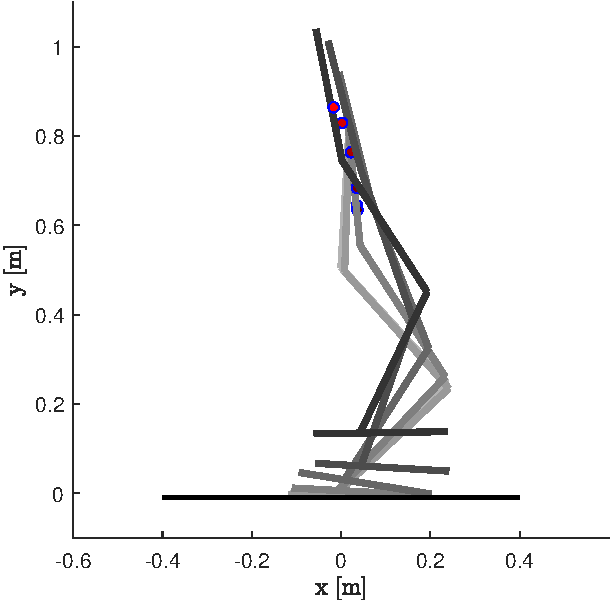
\includegraphics[width=0.6\linewidth]{initialguess}
	}%}	
	\caption{Initial motion used as starting value for the optimisation.}
	\label{fig:seq}	
\end{figure}

\begin{table*}[ht]
	\caption{Jumping optimization results for SEA only, monoarticulated, and biarticulated configurations, respectively.}
	\label{table:maxheight}
	\begin{center}
		\begin{tabular}[t]{c|c|c|c|c|c|c|c|c|c}
			Configuration &  $y_{\text{\textit{CoM}}}^{\text{\textit{max}}}$ [m] & $y_{\text{\textit{CoM}}}^{\text{\textit{initial}}}$ [m]& $y_{\text{\textit{CoM}}}^{\text{\textit{change}}}$ [m]& $p_1,p_2$ [m] & \textit{f} & $E_{\text{\textit{consumed}}}$ [J] & $J_{\text{\textit{performance}}}$ & $J_{\text{\textit{stability}}}$ & $J_{\text{\textit{torque}}}$ \\ 
			\hline
			SEA only	& 0.917 & 0.760 & 0.157 & No \textit{ESB}s	& -370.26 & 805.66 & 426.16 & 0.85 & 55.05\\
			\hline
			Mono.		& 0.951 & 0.703 & 0.247 & 0.060, -0.014	& -402.90 & 567.64 & 451.77 & 1.26 & 47.61 \\
			\hline
			Bi.			& 1.013 & 0.724 & 0.290 & 0.044, 0.029		& -478.73 & 867.35 & 526.27 & 0.96 & 46.58
		\end{tabular}
	\end{center}
\end{table*}


% Large figure with all the optimisation results
\begin{figure*}[ht]
	\centering
	
	% Criteria evolution
	\begin{subfigure}[t]{0.32\linewidth}
		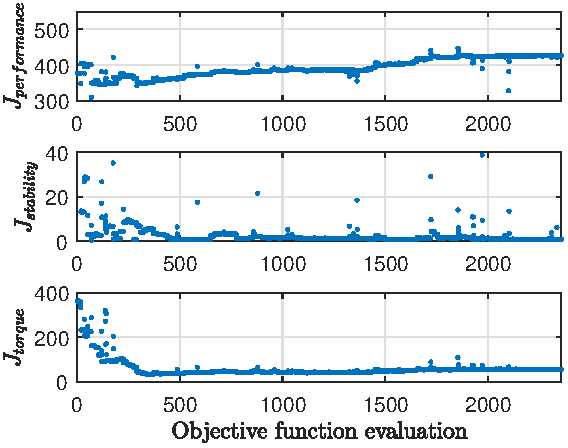
\includegraphics[width=\linewidth]{noESB/crit_high}
		\caption{No ESB: Criterion evolution.}
		\label{fig:noESB_crit_high}
	\end{subfigure}
	%
	\begin{subfigure}[t]{0.32\linewidth}
		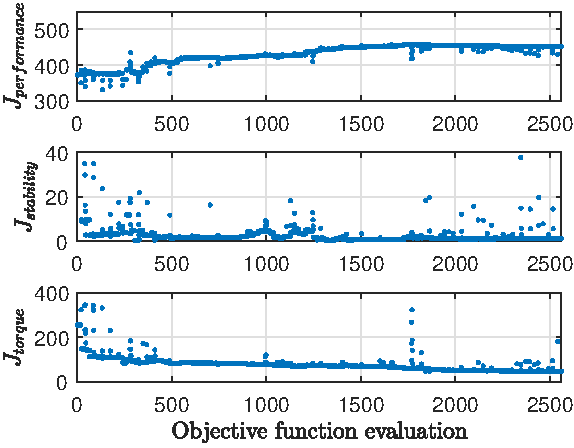
\includegraphics[width=\linewidth]{mono/crit_high}
		\caption{Monoarticulated: Criterion evolution.}
		\label{fig:mono_crit_high}
	\end{subfigure}
	%
	\begin{subfigure}[t]{0.32\linewidth}
		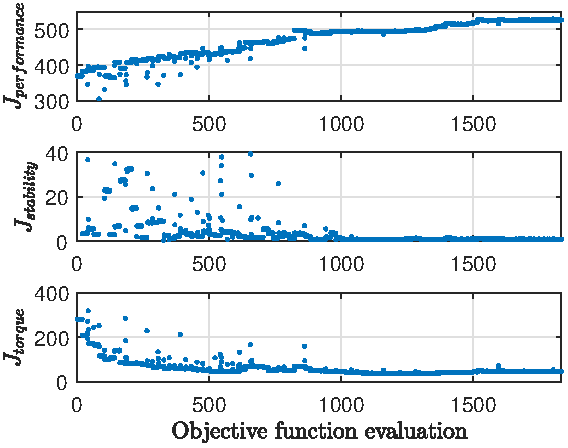
\includegraphics[width=\linewidth]{bi/crit_high}
		\caption{Biarticulated: Criterion evolution.}
		\label{fig:bi_crit_high}
	\end{subfigure}
	
	\vspace{1mm}
	
	% Ankle trajectories
	\begin{subfigure}[t]{0.32\linewidth}
		\includegraphics[width=\linewidth]{noESB/q1_traj}
		\caption{Monoarticulated: Ankle $(q_1)$ trajectory evolution.}
		\label{fig:noESB_q1_traj}
	\end{subfigure}
	%
	\begin{subfigure}[t]{0.32\linewidth}
		\includegraphics[width=\linewidth]{mono/q1_traj}
		\caption{Monoarticulated: Ankle $(q_1)$ trajectory evolution}
		\label{fig:mono_q1_traj}
	\end{subfigure}
	%
	\begin{subfigure}[t]{0.32\linewidth}
		\includegraphics[width=\linewidth]{bi/q1_traj}
		\caption{Biarticulated: Ankle $(q_1)$ trajectory evolution.}
		\label{fig:bi_q1_traj}
	\end{subfigure}
	
	\vspace{1mm}
	
	% Knee trajectories
	\begin{subfigure}[t]{0.32\linewidth}
		\includegraphics[width=\linewidth]{noESB/q2_traj}
		\caption{Monoarticulated: Knee $(q_2)$ trajectory evolution.}
		\label{fig:noESB_q2_traj}
	\end{subfigure}
	%
	\begin{subfigure}[t]{0.32\linewidth}
		\includegraphics[width=\linewidth]{mono/q2_traj}
		\caption{Monoarticulated: Knee $(q_2)$ trajectory evolution}
		\label{fig:mono_q2_traj}
	\end{subfigure}
	%
	\begin{subfigure}[t]{0.32\linewidth}
		\includegraphics[width=\linewidth]{bi/q2_traj}
		\caption{Biarticulated: Knee $(q_2)$ trajectory evolution.}
		\label{fig:bi_q2_traj}
	\end{subfigure}
	
	\vspace{1mm}
	
	% Hip trajectories
	\begin{subfigure}[t]{0.32\linewidth}
		\includegraphics[width=\linewidth]{noESB/q3_traj}
		\caption{Monoarticulated: Hip $(q_3)$ trajectory evolution.}
		\label{fig:noESB_q3_traj}
	\end{subfigure}
	%
	\begin{subfigure}[t]{0.32\linewidth}
		\includegraphics[width=\linewidth]{mono/q3_traj}
		\caption{Monoarticulated: Hip $(q_3)$ trajectory evolution}
		\label{fig:mono_q3_traj}
	\end{subfigure}
	%
	\begin{subfigure}[t]{0.32\linewidth}
		\includegraphics[width=\linewidth]{bi/q3_traj}
		\caption{Biarticulated: Hip $(q_3)$ trajectory evolution.}
		\label{fig:bi_q3_traj}
	\end{subfigure}
	
	\vspace{1mm}
	
	% Ankle torques
	\begin{subfigure}[t]{0.32\linewidth}
		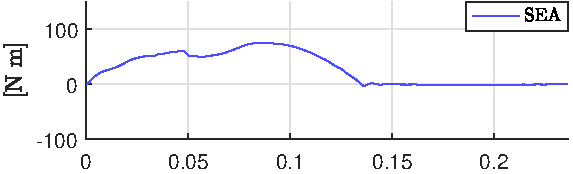
\includegraphics[width=\linewidth]{noESB/q_1_torques}
		\caption{No ESB: Ankle ($q_1$) torques.}
		\label{fig:noESB_q_1_torques}
	\end{subfigure}
	%
	\begin{subfigure}[t]{0.32\linewidth}
		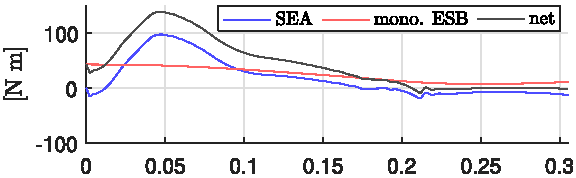
\includegraphics[width=\linewidth]{mono/q_1_torques}
		\caption{Monoarticulated: Ankle ($q_1$) torques.}
		\label{fig:mono_q_1_torques}
	\end{subfigure}
	%
	\begin{subfigure}[t]{0.32\linewidth}
		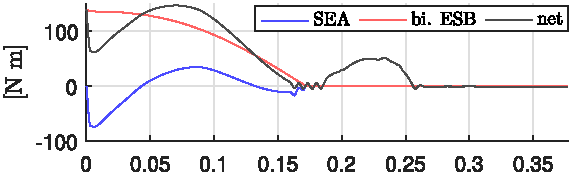
\includegraphics[width=\linewidth]{bi/q_1_torques}
		\caption{Biarticulated: Ankle ($q_1$) torques.}
		\label{fig:bi_q_1_torques}
	\end{subfigure}
	
	\vspace{1mm}
	
	% Knee torques
	\begin{subfigure}[t]{0.32\linewidth}
		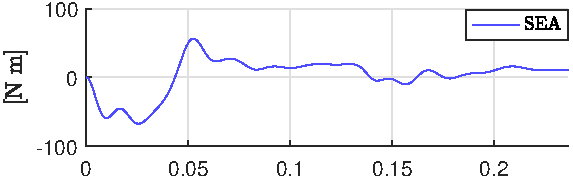
\includegraphics[width=\linewidth]{noESB/q_2_torques}
		\caption{No ESB: Knee ($q_2$) torques.}
		\label{fig:noESB_q_2_torques}
	\end{subfigure}
	%
	\begin{subfigure}[t]{0.32\linewidth}
		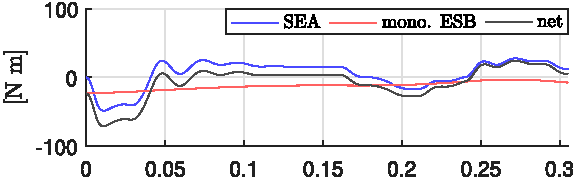
\includegraphics[width=\linewidth]{mono/q_2_torques}
		\caption{Monoarticulated: Knee ($q_2$) torques.}
		\label{fig:mono_q_2_torques}
	\end{subfigure}
	%
	\begin{subfigure}[t]{0.32\linewidth}
		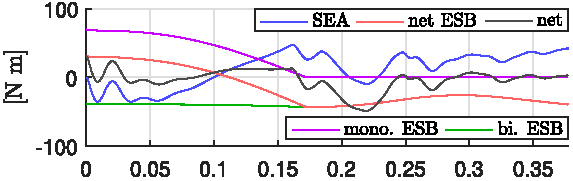
\includegraphics[width=\linewidth]{bi/q_2_torques}
		\caption{Biarticulated: Knee ($q_2$) torques.}
		\label{fig:bi_q_2_torques}
	\end{subfigure}
	
	\vspace{1mm}
	
	% Hip torques
	\begin{subfigure}[t]{0.32\linewidth}
		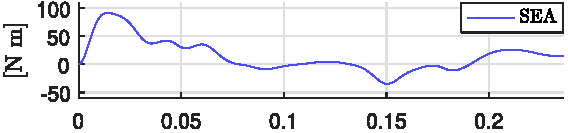
\includegraphics[width=\linewidth]{noESB/q_3_torques}
		\caption{No ESB: Hip ($q_3$) torques.}
		\label{fig:noESB_q_3_torques}
	\end{subfigure}
	%
	\begin{subfigure}[t]{0.32\linewidth}
		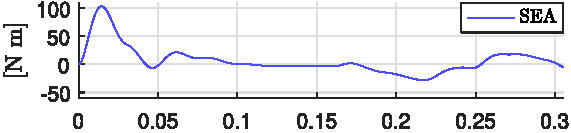
\includegraphics[width=\linewidth]{mono/q_3_torques}
		\caption{Monoarticulated: Hip ($q_3$) torques.}
		\label{fig:mono_q_3_torques}
	\end{subfigure}
	%
	\begin{subfigure}[t]{0.32\linewidth}
		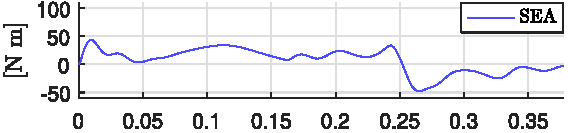
\includegraphics[width=\linewidth]{bi/q_3_torques}
		\caption{Biarticulated: Hip ($q_3$) torques.}
		\label{fig:bi_q_3_torques}
	\end{subfigure}
	
	\vspace{1mm}
	
	% Net Joint power
	\begin{subfigure}[t]{0.32\linewidth}
		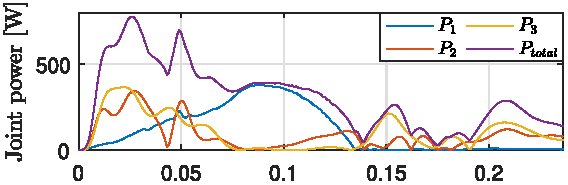
\includegraphics[width=\linewidth]{noESB/P_q}
		\caption{No ESB: Net joint power.}
		\label{fig:noESB_P_q}
	\end{subfigure}
	%
	\begin{subfigure}[t]{0.32\linewidth}
		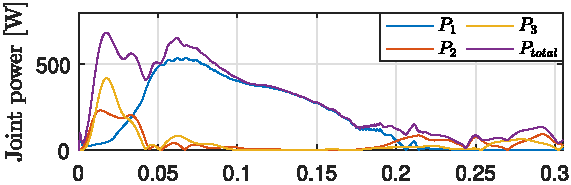
\includegraphics[width=\linewidth]{mono/P_q}
		\caption{Monoarticulated: Net joint power}
		\label{fig:mono_P_q}
	\end{subfigure}
	%
	\begin{subfigure}[t]{0.32\linewidth}
		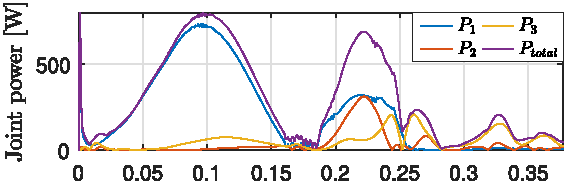
\includegraphics[width=\linewidth]{bi/P_q}
		\caption{Biarticulated: Net joint power}
		\label{fig:bi_P_q}
	\end{subfigure}
	
	\vspace{1mm}
	
	% ESB storage
	\begin{subfigure}[t]{0.32\linewidth}
		\centering
		\raisebox{0pt}[0pt][0pt]{%
			\raisebox{15mm}{\texttt{~~No ESB tendons.}}%
		}
	\end{subfigure}
	%
	\begin{subfigure}[t]{0.32\linewidth}
		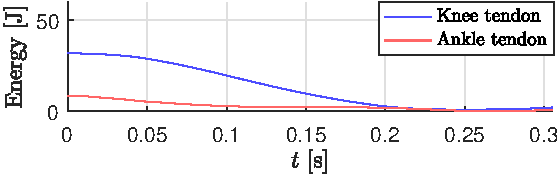
\includegraphics[width=\linewidth]{mono/ESB_storage}
		\caption{Monoarticulated: Tendon energy storage.}
		\label{fig:mono_ESB}
	\end{subfigure}
	%
	\begin{subfigure}[t]{0.32\linewidth}
		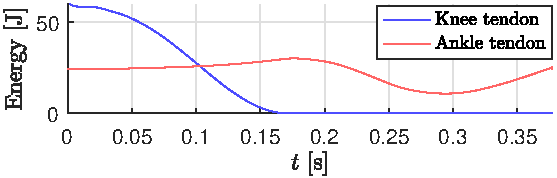
\includegraphics[width=\linewidth]{bi/ESB_storage}
		\caption{Biarticulated: Tendon energy storage.}
		\label{fig:bi_ESB}
	\end{subfigure}
	
	\caption{Optimization results. Left column: without ESB (conventional SEA), middle column: monoarticulated configuration, right column: biarticulated configuration. $A1$ and $A2$ denote the actuators for the ankle joint ($q_1$) and the knee joint ($q_2$), respectively.}
	\label{fig:opt_results}
\end{figure*}


%%%%%%%%%%%%%%%%%%%%%%%%%%%%%%%%%%%%%%%%%%%%%%%%%%%%%%%%%
\section{Discussion} \label{sec:discussion}
%\textbf{TODO comments on the plots:}
%\begin{itemize}
%	\item Can we place the joint trajectory plots for each configuration as well? It seems there is space for one additional row.
%	\item The legend entries currently do not make sense; the symbols were never explained. I'm attaching a few scripts by email (the ones that generated the ICRA18 plots) which have text names for variables that you do not need to explain.
%	\item Somewhat less resampling, plots are very jagged now due to the short displayed time (mentioned in email) 0.005 or 0.0025 (try first) seconds should be fine.
%	\item I would generate the plots a bit smaller, legends are unreadable (there should be a (commented out?) size in the old code for 3 column plots. My standard paper size is [500 190], but in the ICRA18 paper I used [450 230] (a bit higher as there was plenty of y-space). I'll send you the relevant scripts as well.
%\end{itemize}
%\textbf{TODO end plot comments}.

%\textbf{TODO some observations (Wesley):}
%\begin{itemize}
%	\item Strategy of noESB and mono is simular (looking at torque plots), biarticulation allows the bi configuration to adopt a different strategy and reach more height
%	\item Can we see evidence of power transfer from knee to ankle? It appears so; the biarticulated tendon is providing positive torque on the knee (i.e. flexing the knee) for the first 0.17\,s, while the knee is extending. This means positive power is transferred to the ankle (as that linear tendon force translates to a positive torque on the ankle, which extends the ankle, see Fig. \ref{fig:Leg_3DoF_model}). You can also see the stored energy in that tendon stays roughly constant, meaning this energy is not stored but transferred to the ankle. This is great because it is one of the primary arguments of such a configuration.
%\end{itemize}
%\textbf{TODO end observations.}

%\textbf{Some new doodling:}
One immediate observation from the results is that ankle extension is one of the primary contributors to vertical momentum, across all three configurations. This is evidenced by the significantly larger joint power compared to the knee (Fig. \ref{fig:noESB_P_q}--\ref{fig:bi_P_q}). We suspect the reason for this is the relatively large amount of ankle torque available (as identical SEAs are used for ankle and knee), combined with the 0.4\,s maximum duration which may not allow for fully flexed knee at $t=0$. Although the movements for all three configurations are similar, some key differences can be observed:

%\textbf{Earlier text:}
%For the optimised jumping motion similar strategies are used on all three actuation configurations; ankle extension is primarily used to generate an upwards motion from squat position, with lift-off following after a toe push-off. The pretension optimisation results show maximum pretension of the \textit{ESB} on the bottom of the ankle for monoarticulation and the pretension of the \textit{ESB} on the bottom of the thigh for biarticulation. Although the movements are similar some key differences can be pointed out:

\begin{enumerate}
	\item Fig. \ref{fig:noESB_q_1_torques} to \ref{fig:bi_q_1_torques} show that the \textit{PB} ankle torque used by the biarticulated configuration is significantly lower than that of the other configurations but its \textit{ESB} torque is significantly higher than that of the monoarticulated configuration resulting in the heighest ankle torque for biarticulation. 
	
	\item While Fig. \ref{fig:noESB_q_2_torques} shows slightly higher peak \textit{PB} torques for the knee joint than the \textit{ESB} configurations in Fig. \ref{fig:mono_q_2_torques} and \ref{fig:bi_q_2_torques}, knee extension is nearly absent for the configuration without \textit{ESB}. The jumps with mono and biarticulation do show knee extension at approximately 0.2 seconds into the motion. Fig. \ref{fig:bi_q_2_torques} shows that this extension is preceded by counteracting \textit{PB} and \textit{ESB} torques. For the biarticulated configuration the \textit{PB} knee torque counteracts the \textit{ESB} torque after 0.1 seconds, but stops this counteraction instantly which allows for an explosive increase in torque around 0.2 seconds. This allows for explosive knee movement without exceeding torque limits.
	
	\item The limitation by torque restriction for the configuration without \textit{ESB} is implied by Fig. \ref{fig:noESB_crit_high}, which shows an increase in the torque criterion resulting in a higher torque criterion than the legs with \textit{ESB} as shown in Table \ref{table:maxheight}. Restrictions in time and the number of control points may also be an influence on the moderate use of knee joint torque to execute the jump for the configuration without \textit{ESB}.
	
	\item Whereas the configuration without \textit{ESB} and the monoarticulated configuration use hip extension extensively during the early stages of the upwards motion of the jump, Fig. \ref{fig:noESB_q_3_torques} to \ref{fig:bi_q_3_torques} show that the biarticulated configuration uses far less hip extension. The biarticulated leg extends its hip at the end of the upwards motion to increase its CoM height whereas the leg without \textit{ESB} flexes its hip to maintain upwards momentum.
	
	\item Fig. \ref{fig:noESB_P_q} to \ref{fig:bi_P_q} show that the biarticulated configuration net joint power exceeds that of the other configurations. A comparison with Fig. \ref{fig:mono_ESB} and \ref{fig:bi_ESB} shows that for the \textit{ESB} configurations the largest change in power is largely synchronous with release of energy in the \textit{ESB} tendons.
	
\end{enumerate}


%%%%%%%%%%%%%%%%%%%%%%%%%%%%%%%%%%%%%%%%%%%%%%%%%%%%%%%%%
\section{Conclusions} \label{sec:conclusions} 
This paper has presented the trajectory and elastic element pretensions optimisation for the explosive jumping motion of a 3-DoF leg using asymmetric compliant actuators in three different configurations. The results show improvements in terms of torque requirements of the main actuators, as well as interesting collaboration between the elastic elements and the main actuators in order to reach joint torques that allow for explosive motions.

The leg jumps almost 4\% higher with a monoarticulated configuration and over 10\% higher with a biarticulated configuration compared to a configuration without \textit{ESB}.

While these results are promising, experiments with an already existing hardware prototype undergoing mechanical revisions are still to be performed. Also, for this research only fixed pretension positions of the parallel branches have been used. The integration of variable pretension positions may allow for more accurate optimisation. These developments and their results will be presented in future works.


%%%%%%%%%%%%%%%%%%%%%%%%%%%%%%%%%%%%%%%%%%%%%%%%%%%%%%%%%
\addtolength{\textheight}{-0cm}   % This command serves to balance the column lengths
                                  % on the last page of the document manually. It shortens
                                  % the textheight of the last page by a suitable amount.
                                  % This command does not take effect until the next page
                                  % so it should come on the page before the last. Make
                                  % sure that you do not shorten the textheight too much.


%%%%%%%%%%%%%%%%%%%%%%%%%%%%%%%%%%%%%%%%%%%%%%%%%%%%%%%%%
\section{ACKNOWLEDGMENT}
Supported by European Commission projects WALK-MAN (611832), CENTAURO (644839), CogIMon (644727)


%%%%%%%%%%%%%%%%%%%%%%%%%%%%%%%%%%%%%%%%%%%%%%%%%%%%%%%%%
% References
\bibliographystyle{ieeetran} % Requires ieeetran.bst
\bibliography{lit}

\end{document}
